\documentclass{emulateapj}

\usepackage{verbatim}
\usepackage{amsmath}
\usepackage{hyperref}
\usepackage{breakurl}
\usepackage{float}

\usepackage{etoolbox}
\makeatletter
\patchcmd{\@verbatim}
  {\verbatim@font}
  {\verbatim@font\small}
  {}{}
\makeatother

\newcommand{\code}[1]{\texttt{#1}}

\bibliographystyle{apj}

\begin{document}

\title{The Galaxy Cluster Merger Catalog: An Online Repository of Mock Observations from Simulated Galaxy Cluster Mergers}

\author{J. A. ZuHone\altaffilmark{1}, K. Kowalik\altaffilmark{2}}

\altaffiltext{1}{Harvard-Smithsonian Center for Astrophysics, 60 Garden St., Cambridge, MA 02138, USA}
\altaffiltext{2}{National Center for Supercomputing Applications, University of Illinois at Urbana-Champaign, 1205 W. Clark St., MC-257, Urbana, IL 61801, USA}

\begin{abstract}
We present the first release of the ``Galaxy Cluster Merger Catalog''. This catalog provides an extensive suite of mock observations and related data for N-body and hydrodynamical simulations of galaxy cluster mergers. These mock observations consist of projections of a number of important observable quantities in several different wavebands, for the entire evolution of each simulation as well as along different lines of sight through the three-dimensional simulation domain. The web interface to the catalog consists of easily browseable images over epoch and projection direction, as well as download links for the raw data and a JS9 interface for interactive data exploration. All of the data products are provided in the standard FITS file format, in image and table form. Data is being stored on the yt Hub~(\url{https://hub.yt}), which allows for remote access and analysis using Jupyter notebook server. Future versions of the catalog will include simulations from a number of research groups and a variety of research topics related to the study of interactions of galaxy clusters with each other and with their member galaxies. The catalog is located at \url{http://gcmc.hub.yt}.
\end{abstract}

\section{Introduction}\label{sec:intro}

Galaxy clusters are the largest gravitationally bound structures in the current universe. Originally identified as concentrations of galaxies in the optical, observations in the X-ray and millimeter wavelengths have revealed the bulk of baryonic material of clusters is comprised of a hot, magnetized plasma known as the intracluster medium \citep[ICM,][]{for72,sun72}. The kinetic energy of the galaxies and the temperature of the hot gas indicate that in order for the cluster to be gravitationally bound the majority of the mass must be in the form of cold dark matter \citep[CDM, first noted by][]{zwi37}.

Mergers between galaxy clusters represent the latest stage of cosmological structure formation. The most energetic events in the universe, mergers drive shocks and turbulence into the ICM, heating and stirring the cluster gas. These mergers also accelerate relativistic particles, which then produce radio relics and halos \citep{fer05,bru07,vwe10,bru12}. Cluster mergers have also revealed the different dynamical properties of the CDM, galaxies, and ICM, seen most vividly in the case of the Bullet Cluster \citep[][]{clo04,mar04}. Understanding cluster mergers is therefore vital to answering questions about the detailed physics of galaxy clusters as well
as providing insights into the formation of cosmic structure.

The astrophysical literature is replete with simulations of galaxy cluster mergers, from binary merger simulations \citep[e.g.][]{ric01,poo06,zuh11,don13} to studies of mergers in cosmological simulations \citep[e.g.][]{vaz09,ski13,yu15}. These simulations have often attempted to make predictions for what may be observed in a number of wavebands and made direct comparisons to observed merging systems. However, comparing the results of simulations of cluster mergers to these systems is often not straighforward; at what stage are we viewing the merger, and along what line of sight? To make matters more complicated, different combinations of merger epoch and line of sight can produce qualitatively similar projections of cluster emission, making it more difficult to use observations to determine these parameters and distinguish between different theoretical models.

We seek to address these issues by releasing the ``Galaxy Cluster Merger Catalog'', an extensive suite of mock observations and related data for simulations of galaxy cluster mergers. We have produced 2D projections and slices of a number of different quantities relevant to observations of galaxy clusters for a large number of merger simulations. The data products span the important stages of evolution of each merger and a number of relevant projection axes. The goal of this catalog is to provide a way to connect simulations of galaxy cluster mergers with multiwavelength observations of real merging clusters, providing an opportunity for observers to compare clusters in their observations with a particular merging scenario. The data may also be analyzed to make predictions for what various investigations of real clusters may reveal for future observations and missions.

\section{The Data}

\subsection{The Simulations}

At the time of writing, the catalog contains data products from idealized binary cluster merger
simulations. In the future, the catalog will include data products from a variety of galaxy cluster merger and related galaxy cluster simulations, including those from cosmological simulations and simulations of interactions between clusters and their member galaxies. The types of data products are likely to expand and diversify with the inclusion of new simulations.

The galaxy cluster merger simulation data in the catalog comes from state-of-the-art N-body and hydrodynamics codes such as FLASH \citep{dub09} and Athena \citep{sto08}. The exact physics and algorithms employed by the simulations vary, but in general:

\begin{itemize}
\item Each simulation is simulated using an adaptive or static mesh refinement (AMR/SMR) grid \citep{ber89} with varying resolution throughout the domain, with refinement occuring on criteria such as sharp jumps in density and temperature, matter density, and selected regions such as the cluster center.
\item The equations of hydrodynamics (HD) or magnetohydrodynamics (MHD) are modeled using a conservative finite-volume scheme, employing Riemann solvers for evolving the flux of physical quantities and using high-order reconstruction schemes such as the Piecewise-Parabolic Method \citep[PPM,][]{col84}. If present, magnetic fields are evolved such that the condition $\nabla \cdot {\bf B} = 0$ is met, typically by a constrained transport scheme \citep[CT,][]{eva88}.
\item Each simulation assumes an ideal gas law equation of state with $\gamma = 5/3$ and primordial abundances of H/He with trace amounts of metals, yielding a mean molecular weight of $\mu \simeq 0.6$.
\item If dark matter is included, it is modeled by an N-body solver for a collection of collisionless massive particles, which interact with the gas component only via gravity.
\item The gravity in the simulations is either modeled as a rigid gravitational potential associated with each cluster or by computing the self-gravity of the gas and dark matter using a Poisson solver \citep[e.g.,][]{ric08}.
\item Depending on the goals of the simulation study, other physics, such as viscosity, thermal conduction, radiative cooling, etc., may be included.
\end{itemize}

Though currently the simulations represented in the catalog are of the grid-based variety, eventually the catalog will also include data from smoothed particle hydrodynamics (SPH) simulations.

\subsection{Methods and Technologies}\label{sec:methods}

In this section, we briefly outline the methods and software used to generate the data products from the original simulation data and host them on the catalog website.

\subsubsection{Python Scientific Software}\label{sec:software}

The projected data is generated from the original simulation data using yt \citep{tur11}, an open-source Python package for analyzing and visualizing volumetric data. yt has capabilities for slicing and projecting physical fields from multi-resolution datasets such as those from galaxy cluster merger simulations along arbitrary lines of sight. Through analysis modules and affiliated packages, yt also has capabilities to produce synthetic Sunyaev-Zeldovich (S-Z) and X-ray observations. We provide details on how this is done in Sections \ref{sec:sz} and \ref{sec:xray}.

AstroPy \citep{apy13} is used to take the projected data generated in yt and produce data outputs in the standard Flexible Image Transport System (FITS) data format \citep{pen10} and generate coordinates for the files using the World Coordinate System \citep[WCS,][]{gre02, cal02} specification.

\subsubsection{JS9}\label{sec:js9}

JS9 (\url{http://js9.si.edu}) is a browser-based implementation of SAOImage DS9 (\url{http://ds9.si.edu/}), an astronomical imaging and data visualization application. JS9 provides interactive exploration of FITS image and table data including zooming, panning, colormaps, scaling, and region files. On each ``epoch page'' (Section \ref{sec:epoch_page}) there is an interface to JS9 and links to open FITS files from that epoch in the JS9 interface.

\subsubsection{The yt Hub}\label{sec:yt_hub}
The catalog data is stored on the \code{yt Hub}\footnote{\url{https://hub.yt/}}, a conglomerate of various open source
services creating an environment that allows one to collect, remotely analyze, share and publish scientific datasets. At
its core, the \code{yt Hub} uses \code{Girder}\footnote{\url{https://girder.readthedocs.io}}, a data management platform
that allows to transparently store, serve, and proxy data from heterogeneous backend storage engines through a single
web API. Data served by \code{Girder} can easily be gathered into dynamical hierarchies such as collections, folders and
items.  This data management system is integrated with
\code{JupyterHub}\footnote{\url{https://jupyterhub.readthedocs.io/}} and allows authenticated users to spawn Jupyter
notebook servers with direct access to the data that is provided as a dynamically composed FUSE filesystem. Any Jupyter
notebook created in that environment during an interactive session is safely stored back in the \code{Girder} instance,
preserving the user's analysis workflow and increasing research reproducibility. In the future, we plan to have this
notebook capability integrated directly with the catalog website.

\subsection{The Data Products}\label{sec:data}

The data products currently provided in the catalog are 2D selections or reductions of the original 3D datasets, such as slices or projections. The particular products included for a particular simulation depend on its physical and algorithmic details (e.g., slices of the magnetic field strength and Faraday rotation measure projections are only included for MHD simulations).

The data products are all written in the FITS format, in image and table form. Each FITS file may contain more than one image or table extension. The header of each extension contains coordinate information stored using standard WCS keywords. Each FITS file contains one or both of the following two coordinate systems:

\begin{itemize}
\item A linear coordinate system which corresponds to the coordinate system of the original dataset. The length units are in kpc. For most of the FITS files, this is the first and primary WCS (e.g., the one that appears by default in ds9).
\item A celestial coordinate system in RA and Dec using the tangential projection. The angle units are in degrees. For most of the FITS files, this is the secondary WCS (e.g., ``WCS a'' in ds9).
\end{itemize}

For example, a header for one of the FITS images corresponding to a projected quantity may look like this (omitting some keywords for clarity):

\begin{verbatim}
NAXIS   =                    2
NAXIS1  =                 2048
NAXIS2  =                 2048
EXTNAME = 'KT      '
BTYPE   = 'kT      '
BUNIT   = 'keV     '
WCSAXES =                    2
CRPIX1  =               1024.5
CRPIX2  =               1024.5
CDELT1  =     0.97653794699453
CDELT2  =     0.97653794699453
CUNIT1  = 'kpc     '
CUNIT2  = 'kpc     '
CTYPE1  = 'LINEAR  '
CTYPE2  = 'LINEAR  '
CRVAL1  =                  0.0
CRVAL2  =                  0.0
LATPOLE =                 90.0
WCSNAME = 'yt      '
WCSAXESA=                    2
CRPIX1A =               1024.5
CRPIX2A =               1024.5
CDELT1A = -0.00028118222874698
CDELT2A =  0.00028118222874698
CUNIT1A = 'deg     '
CUNIT2A = 'deg     '
CTYPE1A = 'RA---TAN'
CTYPE2A = 'DEC--TAN'
CRVAL1A =                 30.0
CRVAL2A =                 45.0
LONPOLEA=                180.0
LATPOLEA=                 45.0
WCSNAMEA= 'celestial'
RADESYSA= 'ICRS    '
TIME    =    1.300254073176463
\end{verbatim}

It can be seen here that the default WCS, \code{WCSNAME = 'yt'}, is in linear coordinates, and the second WCS, \code{WCSNAMEA = 'celestial'}, is in celestial coordinates. The relationship between the two depends on the angular diameter distance to the source, which depends on the redshift and the given cosmology. The pixel scale of each FITS file is equivalent to the finest cell size of the simulation.

With the exception of the X-ray event files (Section \ref{sec:xray}), no attempt is made in the mock observations to include statistical and systematic errors on the observed quantities, instrumental effects, or background contamination. It is not possible to anticipate in advance what assumptions the end-user may want to make about these issues, so these effects have been left out so they may be added on a case-by-case basis for different situations.

The next several subsections describe in detail the types of data products.

\subsubsection{Slices}\label{sec:slices}

Each simulation epoch has a FITS file containing slices through the central merger plane of a subset of the following fields, contained within different HDUs with the following extension names:

\begin{itemize}
\item \code{"density"}: Gas density in units of $\rm{M_\odot~kpc^{-3}}$.
\item \code{"dark\_matter\_density"}: Dark matter density in units of $\rm{M_\odot~kpc^{-3}}$.
\item \code{"kT"}: Gas temperature in units of keV.
\item \code{"velocity\_x"}: The x-component of the gas velocity in units of $\rm{km~s^{-1}}$.
\item \code{"velocity\_y"}: The y-component of the gas velocity in units of $\rm{km~s^{-1}}$.
\item \code{"magnetic\_field\_strength"}: The magnetic field strength in units of $\mu$G.
\end{itemize}

For a number of the simulations, fields representing the mass fraction of gas from each cluster within a particular cell are also included. The header for each image includes a linear WCS with distances given in kpc. These slices can be used to examine the history of the merger from the perspective of the 3D physical quantities which are evolved by the simulation, and from which the 2D projected quantities are derived.

\subsubsection{Projections}\label{sec:projections}

\begin{figure*}
\begin{center}
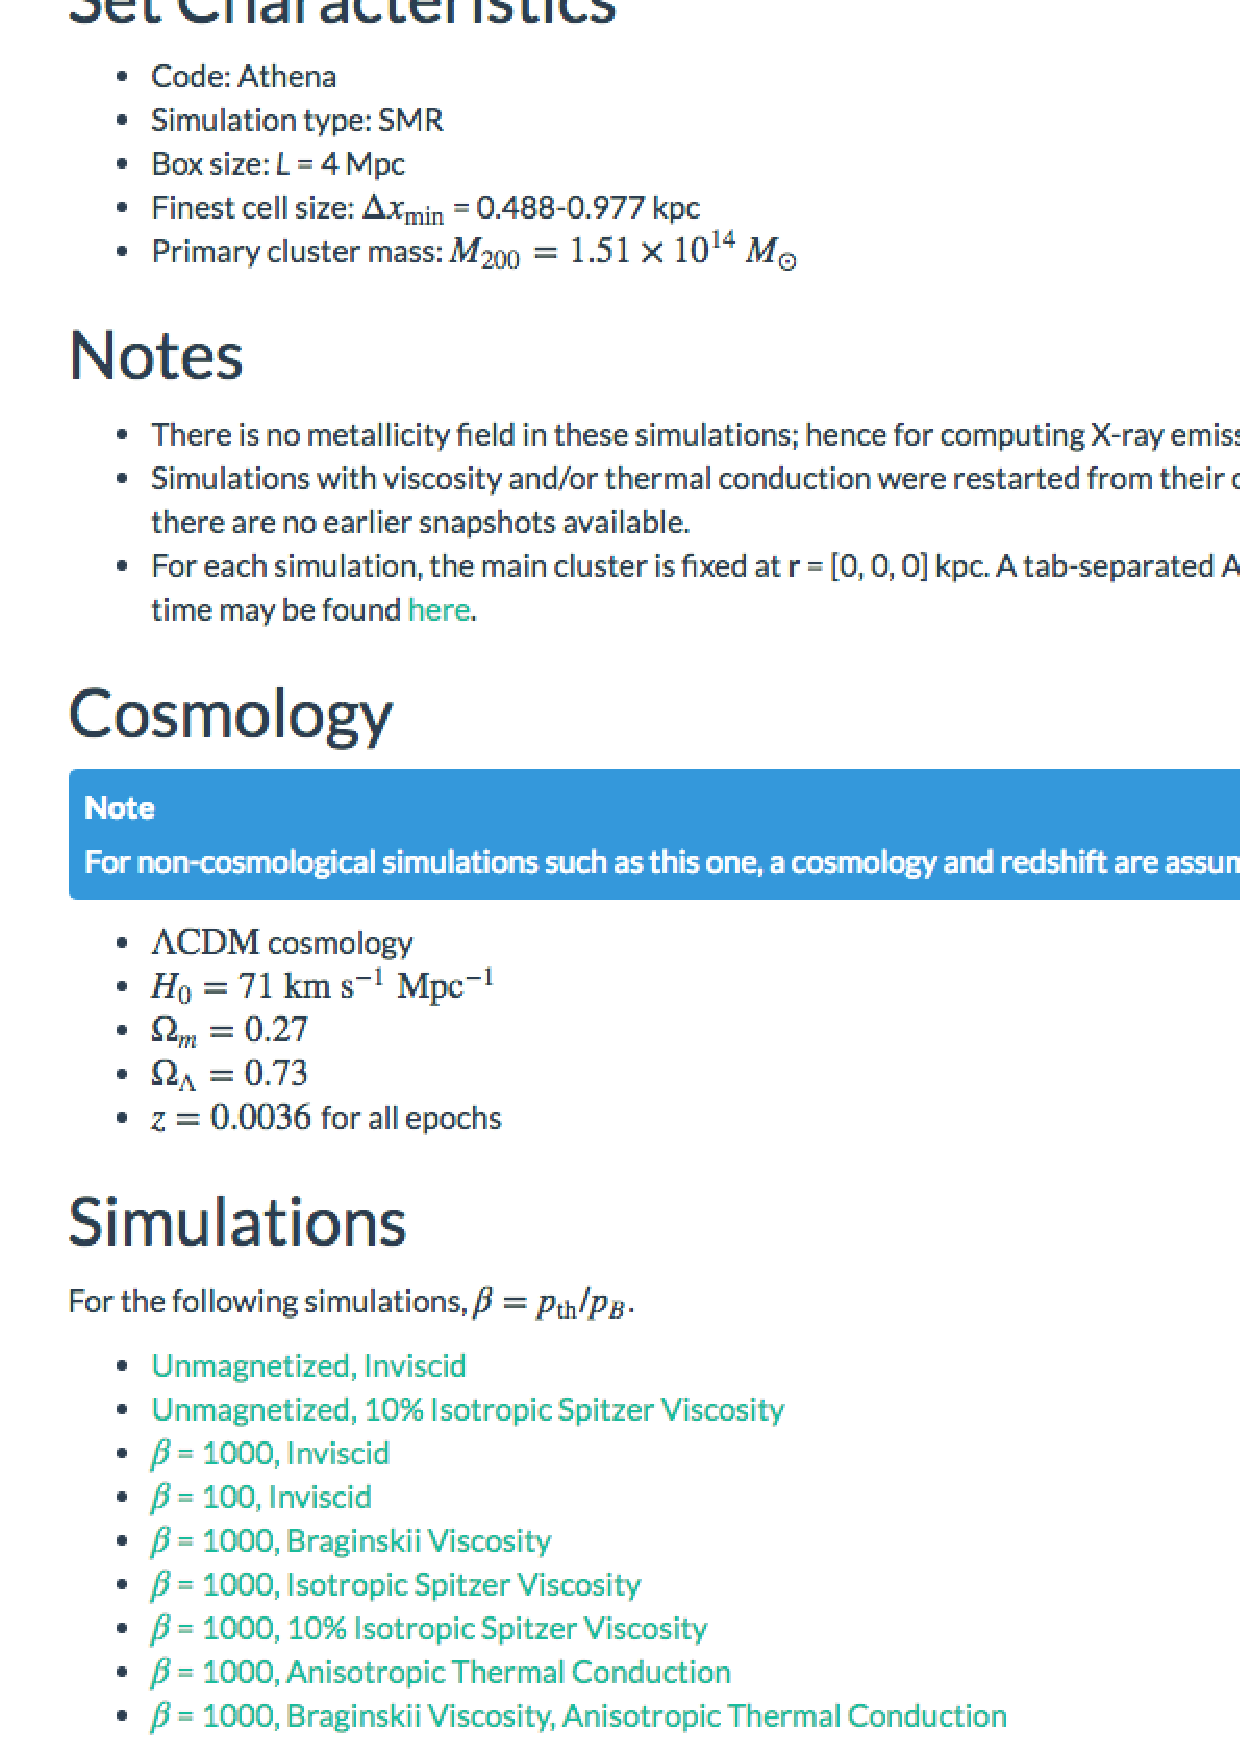
\includegraphics[width=0.9\textwidth]{set_page.png}
\caption{An example ``set page''. Links are provided to original journal articles, various simulation parameters and other information are tabulated, and links to the data for the individual simulations appear here. This particular page is linked at \url{http://gcmc.hub.yt/virgo/index.html}.}
\end{center}
\end{figure*}

\begin{figure*}
\begin{center}
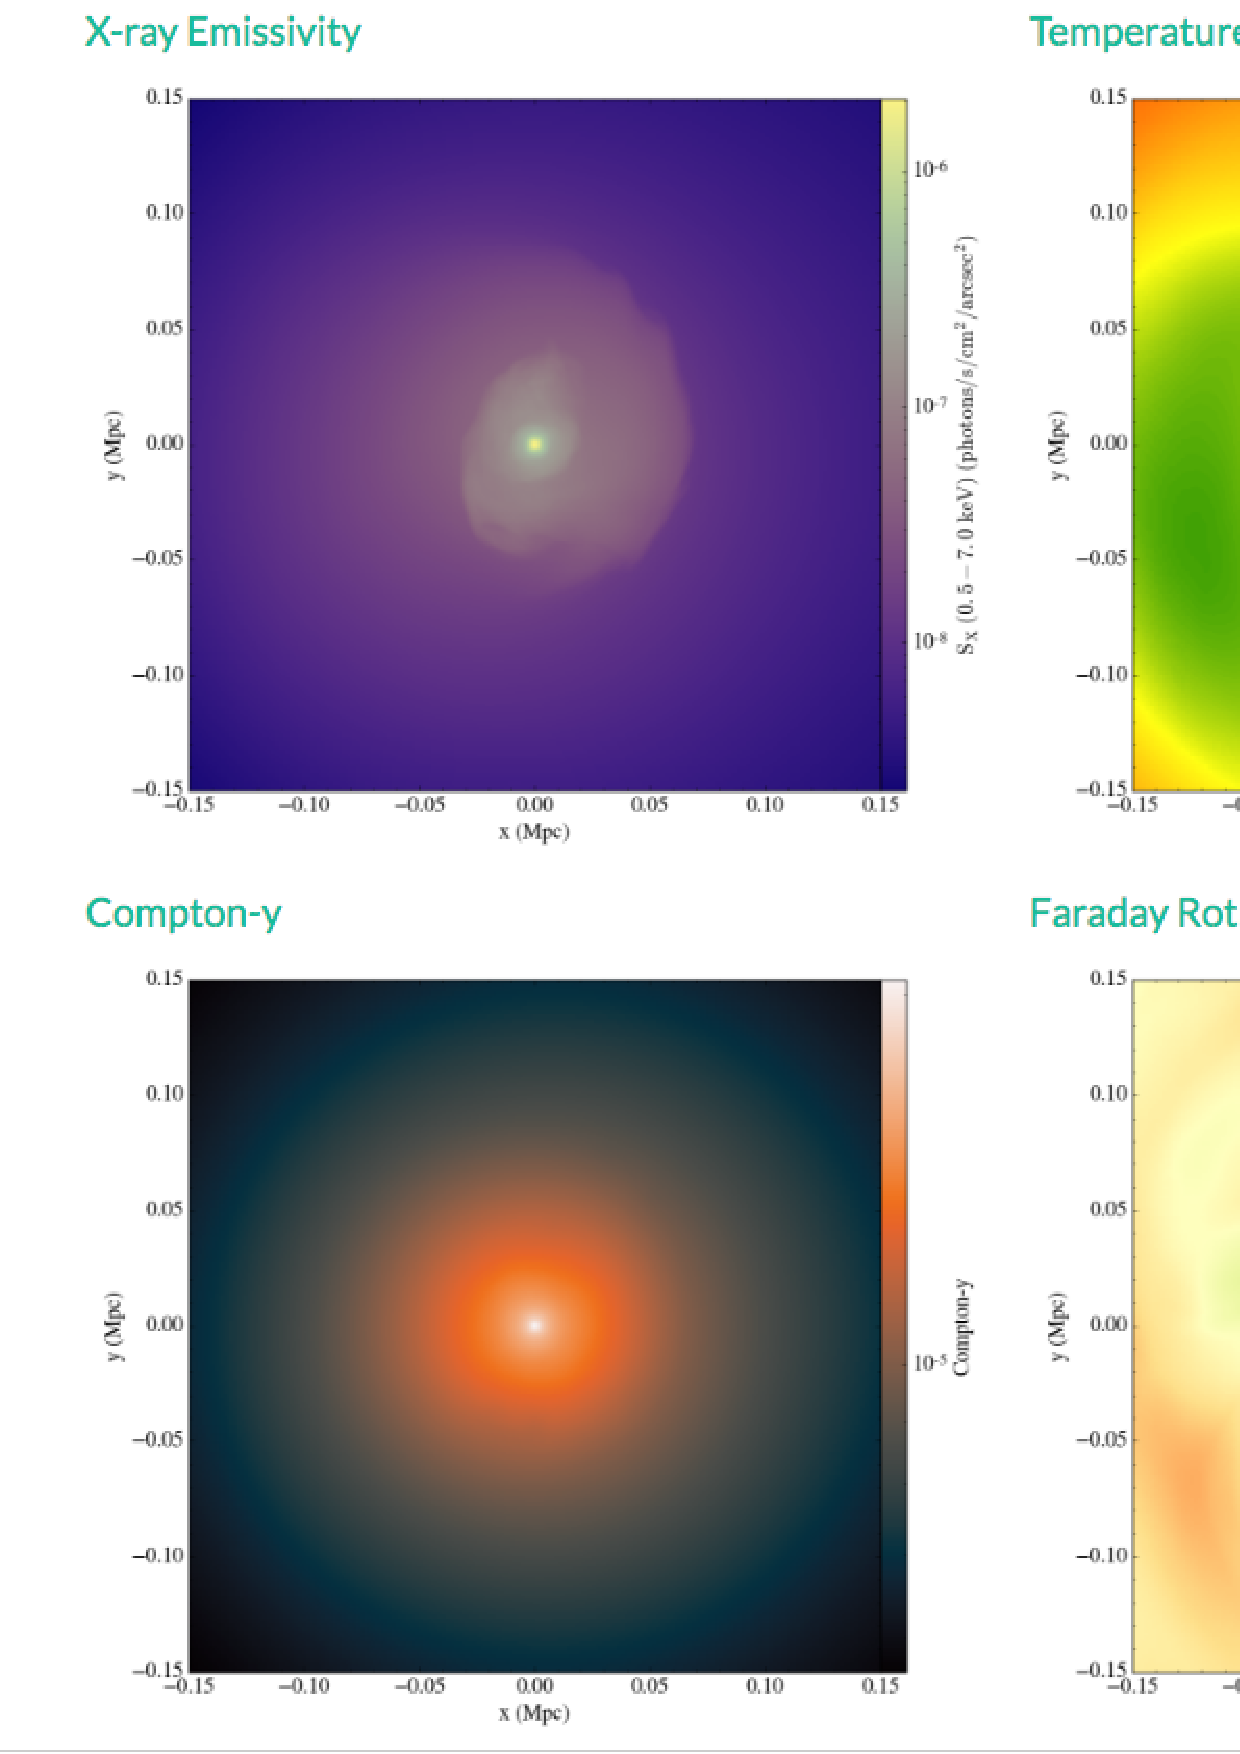
\includegraphics[width=0.9\textwidth]{sim_page.png}
\caption{An example ``simulation page''. Slider bars allow exploration of different epochs, and buttons near the top choose different projection axes. The figures link to the page for the files for the corresponding epoch of the simulation. This particular page is linked at \url{http://gcmc.hub.yt/virgo/novisc/index.html}.}
\end{center}
\end{figure*}

\begin{figure*}
\begin{center}
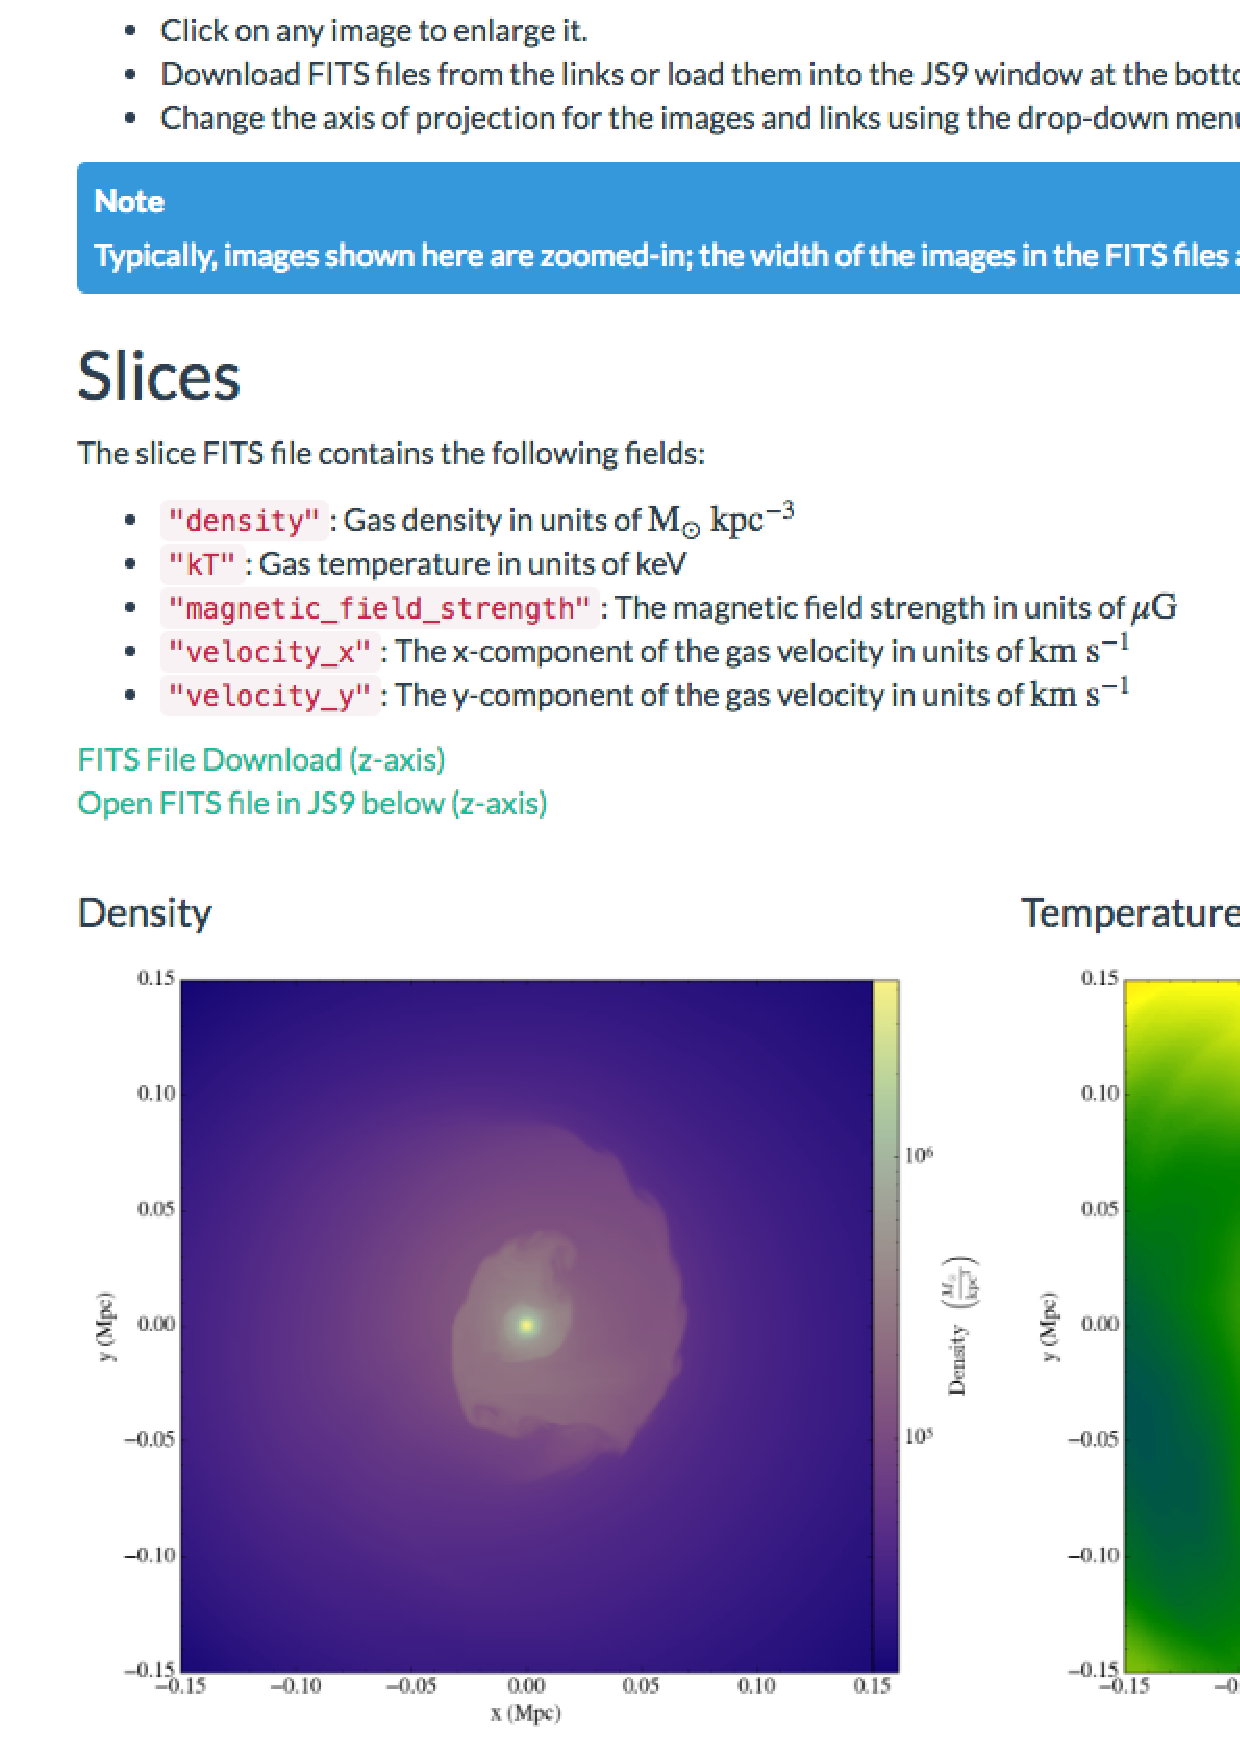
\includegraphics[width=0.9\textwidth]{epoch_page.png}
\caption{An example ``epoch page''. Links are provided to similar simulations with different physics at the same epoch at the top of the page. For each data type, figures of some of the fields are shown and links to download the data or display in JS9 are provided. This particular page is linked at \url{http://gcmc.hub.yt/virgo/novisc/0046/index.html}.}
\end{center}
\end{figure*}

\begin{figure*}
\begin{center}
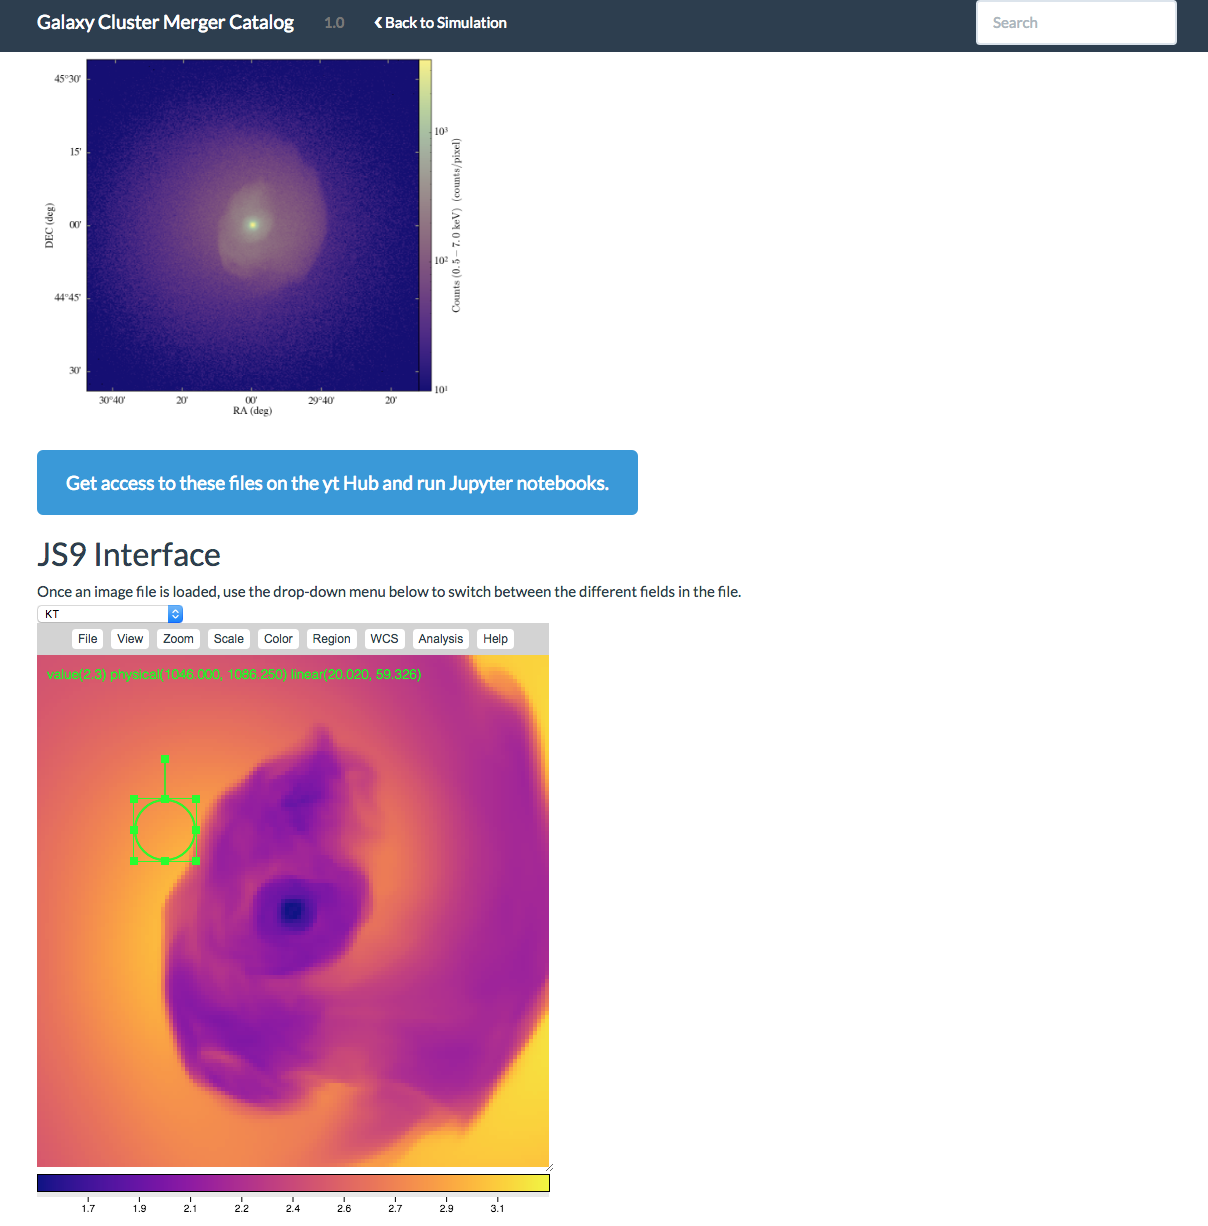
\includegraphics[width=0.9\textwidth]{epoch_page2.png}
\caption{The bottom of an ``epoch page'', showing the simulated X-ray event file and the JS9 interface with a projection file loaded, and a circular region selected. This particular page is linked at \url{http://gcmc.hub.yt/virgo/novisc/0046/index.html}.}
\end{center}
\end{figure*}

Projections are taken along several lines of sight. Currently, these include the three major axes of the simulation domain: $x$, $y$, and $z$. In the future, projections along off-axis directions will be added. For distance and redshift-dependent quantities, each simulation employs either the cosmology and redshift from the simulation, or for simulations without such information, a redshift and a $\Lambda{\rm CDM}$ cosmology is assumed with the following parameters: $H_0 = 71~{\rm km~s^{-1}~Mpc^{-1}},$ $\Omega_m = 0.27$, and $\Omega_\Lambda = 0.73$. The projection files each have a subset of the following fields contained within different HDUs with the following extension names:

\begin{itemize}
\item \code{"xray\_emissivity"}: X-ray photon surface brightness in the 0.5-7.0~keV (observer) band, computed using an APEC model, in units of ${\rm photons~s^{-1}~{cm}^{-2}~{arcsec}^{-2}}$. For simulations without metallicity, a spatially constant metallicity of ${\rm Z = 0.3~Z_\odot}$ is assumed.
\item \code{"kT"}: Emission-weighted projected temperature, using the emissivity described above, in units of keV.
\item \code{"total\_density"}: Total mass density (gas and dark matter) in units of $\rm{M_\odot~{kpc}^{-3}}$.
\item \code{"szy"}: The integrated ``y-parameter'' for the thermal S-Z effect, given by
\begin{equation}
y_{\rm tSZ} = \int{\frac{k_BT}{m_e{c^2}}\sigma_T{n_e}{\rm d\ell}}.
\end{equation}
\item \code{"sz\_kinetic"}: The integrated ``y-parameter'' for the kinetic S-Z effect, given by
\begin{equation}
y_{\rm kSZ} = \int{\frac{v_\ell}{c}\sigma_T{n_e}{\rm d\ell}}.
\end{equation}
\item \code{"rotation\_measure"}: Faraday rotation measure in units of rad~m$^{-2}$, given by:
\begin{equation}
{\rm RM} = \frac{e^3}{2\pi{m_e}^2c^4}\int{n_e}{B_{\ell}}{\rm d}{\ell}.
\end{equation}
\end{itemize}

\subsubsection{Sunyaev-Zeldovich Effect Projections}\label{sec:sz}

Projections of the full S-Z signal are also computed for some simulations, using the \code{SZpack}\footnote{\url{http://www.cita.utoronto.ca/~jchluba/Science_Jens/SZpack/SZpack.html}} library \citep{chl12, chl13} to compute the S-Z signal, including thermal and kinetic contributions as well as relativistic corrections. More details on how these projections were computed can be found at \url{http://yt-project.org/doc/analyzing/analysis_modules/sunyaev_zeldovich.html}. They are stored in separate FITS files from the other projections. Currently, these files contain a subset of these fields with the follwing extension names:

\begin{itemize}
\item \code{"Tau"}: Compton optical depth of the cluster gas
\item \code{"TeSZ"}: Mass-weighted projected temperature in units of keV
\item \code{"90\_GHz"}: S-Z signal at 90~GHz in units of MJy~sr$^{-1}$
\item \code{"180\_GHz"}: S-Z signal at 180~GHz in units of MJy~sr$^{-1}$
\item \code{"240\_GHz"}: S-Z signal at 240~GHz in units of MJy~sr$^{-1}$
\end{itemize}

The computed S-Z signal at other frequencies may be added in later revisions of the catalog.

\subsubsection{X-ray Event Files}\label{sec:xray}

The X-ray emissivity projection listed above represents a single broad energy band from 0.5-7.0 keV. However, to do analysis of the thermal and compositional properties of the ICM, high-resolution energy spectra are required. Instead of providing similar maps at the same spatial resolution for hundreds or even thousands of energy bins for every epoch and projection direction, which would be prohibitive in terms of disk space, the catalog provides event files.

These X-ray event files are standard products which can be manipulated and analyzed with common X-ray analysis tools, such as ds9, \code{CIAO}, and the \code{HEASOFT} software suite. The events themselves have been generated from the original 3-D datasets using the \code{pyXSIM}\footnote{\url{http://hea-www.cfa.harvard.edu/~jzuhone/pyxsim}} package \citep{zuh14}, which not only generates the 2-D projected X-ray events but can also convolve the photons with instrumental response matrices. At the time of writing, event files for the {\it Chandra} ACIS-I detector are provided, but eventually event files for other instruments will be included, as well as raw, unconvolved events which may be used as input for any instrument simulator.

The event files are designed to provide approximate representations of real observations, with some simplifications. First, the event energies have been convolved with the ACIS-I on-axis responses over the entire field of view. Second, the pixel size corresponds to the width of the finest simulation cell size (in line with the other data products), instead of the pixel scale of the detector. Thirdly, since the {\it Chandra} PSF is very small and for the distances assumed here the cell sizes are typically much larger, no PSF effects have been applied. The idea is not to create an exact simulation, but instead to approximate the statistical properties of the source while allowing one to use standard X-ray tools to analyze the spectral and spatial properties of the data.

\subsubsection{Mock Galaxy Catalogs}\label{sec:galaxies}

A number of the simulations have been run using an N-body code to represent the collisionless dark matter component of the cluster via massive particles. A number of these dark matter particles can be sampled from the simulation to represent mock ``galaxies'', which can also be treated as a collisionless component. For some of these simulations, we have created mock galaxy catalogs.

A number of particles are drawn from each halo within a radius of $r_{200}$, determined by the mass-richness relation of \citet{for14}, from the intitial simulation epoch, which are the ``galaxies''. The same galaxy particles are tracked for the rest of the epochs in the simulation. The FITS binary tables for the galaxies include sky positions, line-of-sight velocities, an identifier for which halo each galaxy originally belonged to, and unique IDs for every galaxy. These particles provide a way of measuring the kinematics of the merger from the perspective of the collisionless material with a statistical significance that is comparable to that obtained from measured redshifts of member galaxies in real clusters. No redshift errors have been applied to the galaxy velocities, which is an exercise left to the end-user.

A ds9 region file containing point regions corresponding to the galaxy positions is provided for each epoch and line-of-sight in addition to the FITS file, which allows the galaxy positions to be plotted over the projections of the other fields.

\subsection{The Interface}\label{sec:interface}

The web interface to the catalog is designed to provide straightforward interactive browsing of a given simulation's data across its many epochs and between several projection axes. This facilitates comparisons between the mock observations and actual observations of clusters so that a potential analog of a particular system may be found easily.

The portion of the website containing the simulation data is structured using the following hierarchy of pages, described in the next few subsections.

\subsubsection{The Set Page}\label{sec:set_page}

The ``set page'' describes the general characteristics of a single set of simulations from a particular investigation and provides links to the individual simulations. This page also provides links to original journal articles which the simulation data appeared in, as well as basic characteristics of the simulation data including the size of the domain, the finest cell size, the characteristic mass of the clusters, etc. This page may also include links to supplementary data files that are common to all of the simulations in the set.

All of the set pages are linked from the main simulation page, which can be found at \url{http://gcmc.hub.yt/simulations.html}.

\subsubsection{The Simulation Page}\label{sec:sim_page}

Every simulation of a set has a ``simulation page'' which shows various quantities projected perpendicular to the merger plane for every epoch of the simulation that is available. The different epochs can be navigated using a slider bar, and buttons above the slider bar can be used to look at the same images from a different line of sight. The links attached to the images lead to the epoch pages.

\subsubsection{The Epoch Page}\label{sec:epoch_page}

Any given link on the simulation page leads to an ``epoch page'' where images from a particular simulation epoch can be examined and the corresponding data may be obtained. Links are provided to similar simulations with different input physics at the same epoch. This page also contains information about the different types of data within the files. A drop-down menu is provided for switching between the different projection axes available.

Each epoch page also contains a JS9 application for opening the various FITS files associated with that particular epoch. A drop-down menu is provided for navigating between the various fields in each FITS file.

\section{Summary}\label{sec:summary}

We have made the first release of the ``Galaxy Cluster Merger Catalog'', a website designed to provide a simple yet powerful interface to accessing mock observations of galaxy cluster mergers. This release includes a suite of mock observations from a number of binary cluster merger simulations, with different initial conditions and input physics. In particular, the catalog provides a number of X-ray and S-Z synthetic observations as well as mock galaxy catalogs. Projections of the observables have been taken along a number of lines of sight through the simulation box, and at a large number of epochs for each simulation so that the merger history is well-sampled in time. This large parameter space of cluster mergers will be useful when comparing with observed cluster mergers in a number of wavebands. 

The catalog is designed so that it may be easily extended and expanded. Future goals include:

\begin{itemize}
\item Adding cluster merger simulations from other research groups, especially those from cosmlogical simulations
\item Adding mock observations from other wavebands, such as radio and optical
\item Adding additional lines of sight through the simulation domain
\item Implementing more ways to interact with the data, such as Jupyter notebooks that may be run on the server
\item Adding other types of data products, including movies, unconvolved X-ray event lists, and the original 3D datasets
\item Providing example scripts to show other researchers how to generate similar data products from their simulations
\end{itemize}

It is our hope that the catalog will provide a useful resource for researchers studying galaxy cluster mergers from both the perspective of current observations as well as making predictions for future missions.

\acknowledgements
JAZ thanks Eric Mandel for tips on using JS9 and for critical bug fixes and enhancements that were provided to make it work with the data in the catalog. JAZ acknowledges support through Chandra Award Number G04-15088X issued by the Chandra X-ray Center, which is operated by the Smithsonian Astrophysical Observatory for and on behalf of NASA under contract NAS8-03060.
KK was funded in part by the Gordon and Betty Moore Foundation's Data-Driven Discovery Initiative through Grant GBMF4561.

\begin{thebibliography}{}
\bibitem[Astropy Collaboration et al.(2013)]{apy13} Astropy Collaboration, Robitaille, T.~P., Tollerud, E.~J., et al.\ 2013, \aap, 558, A33
\bibitem[Berger \& Colella(1989)]{ber89} Berger, M.~J., \& Colella, P.\ 1989, Journal of Computational Physics, 82, 64
\bibitem[Br{\"u}ggen et al.(2012)]{bru12} Br{\"u}ggen, M., Bykov, A., Ryu, D., R{\"o}ttgering, H.\ 2012, \ssr, 166, 187
\bibitem[Brunetti \& Lazarian(2007)]{bru07} Brunetti, G., \& Lazarian, A.\ 2007, \mnras, 378, 245
\bibitem[Colella \& Woodward(1984)]{col84} Colella, P., \& Woodward, P.~R.\ 1984, Journal of Computational Physics, 54, 174
\bibitem[Greisen \& Calabretta(2002)]{gre02} Greisen, E.~W., \& Calabretta, M.~R.\ 2002, \aap, 395, 1061
\bibitem[Calabretta \& Greisen(2002)]{cal02} Calabretta, M.~R., \& Greisen, E.~W.\ 2002, \aap, 395, 1077
\bibitem[Clowe et al.(2004)]{clo04} Clowe, D., Gonzalez, A., \& Markevitch, M.\ 2004, \apj, 604, 596
\bibitem[Chluba et al.(2012)]{chl12} Chluba, J., Nagai, D., Sazonov, S., \& Nelson, K.\ 2012, \mnras, 426, 510
\bibitem[Chluba et al.(2013)]{chl13} Chluba, J., Switzer, E., Nelson, K., \& Nagai, D.\ 2013, \mnras, 430, 3054
\bibitem[Donnert et al.(2013)]{don13} Donnert, J., Dolag, K., Brunetti, G., \& Cassano, R.\ 2013, \mnras, 429, 3564
\bibitem[{Dubey} et~al.(2009)]{dub09} {Dubey}, A., {Antypas}, K.,
  {Ganapathy}, M.~K., {Reid}, L.~B., {Riley}, K.~M., {Sheeler}, D.,
  {Siegel}, A., {Weide}, K. Extensible component based architecture
  for FLASH, a massively parallel, multiphysics simulation
  code. Parallel Computing 35~(10-11), 512--522.
\bibitem[Evans \& Hawley(1988)]{eva88} Evans, C.~R., \& Hawley, J.~F.\ 1988, \apj, 332, 659
\bibitem[Feretti(2005)]{fer05} Feretti, L.\ 2005, Advances in Space Research, 36, 729
\bibitem[Ford et al.(2014)]{for14} Ford, J., Hildebrandt, H., Van Waerbeke, L., et al.\ 2014, \mnras, 439, 3755
\bibitem[Forman et al.(1972)]{for72} Forman, W., Kellogg, E., Gursky, H., Tananbaum, H., \& Giacconi, R.\ 1972, \apj, 178, 309
\bibitem[Markevitch et al.(2004)]{mar04} Markevitch, M., Gonzalez, A.~H., Clowe, D., et al.\ 2004, \apj, 606, 819
\bibitem[Pence et al.(2010)]{pen10} Pence, W.~D., Chiappetti, L., Page, C.~G., Shaw, R.~A., \& Stobie, E.\ 2010, \aap, 524, A42
\bibitem[Poole et al.(2006)]{poo06} Poole, G.~B., Fardal, M.~A., Babul, A., McCarthy, I.~G., Quinn, T., \& Wadsley, J.\ 2006, \mnras, 373, 881
\bibitem[Ricker \& Sarazin(2001)]{ric01} Ricker, P.~M., \& Sarazin, C.~L.\ 2001, \apj, 561, 621
\bibitem[Ricker(2008)]{ric08} Ricker, P.~M.\ 2008, \apjs, 176, 293-300
\bibitem[Skillman et al.(2013)]{ski13} Skillman, S.~W., Xu, H., Hallman, E.~J., et al.\ 2013, \apj, 765, 21
\bibitem[Stone et al.(2008)]{sto08} Stone, J.~M., Gardiner, T.~A., Teuben, P., Hawley, J.~F., \& Simon, J.~B.\ 2008, \apjs, 178, 137
\bibitem[Sunyaev \& Zeldovich(1972)]{sun72} Sunyaev, R.~A., \& Zeldovich, Y.~B.\ 1972, Comments on Astrophysics and Space Physics, 4, 173
\bibitem[Turk et al.(2011)]{tur11} Turk, M.~J., Smith, B.~D., Oishi, J.~S., Skory, S., Skillman, S.~W., Abel, T., \& Norman, M.~L.\ 2011, \apjs, 192, 9
\bibitem[van Weeren et al.(2010)]{vwe10} van Weeren, R.~J., R{\"o}ttgering, H.~J.~A., Br{\"u}ggen, M., \& Hoeft, M.\ 2010, Science, 330, 347
\bibitem[Vazza et al.(2009)]{vaz09} Vazza, F., Brunetti, G., Kritsuk, A., et al.\ 2009, \aap, 504, 33
\bibitem[Yu et al.(2015)]{yu15} Yu, L., Nelson, K., \& Nagai, D.\ 2015, \apj, 807, 12
\bibitem[ZuHone et al.(2010)]{zuh10} ZuHone, J.~A., Markevitch, M., \& Johnson, R.~E.\ 2010, \apj, 717, 908 (ZMJ10)
\bibitem[ZuHone(2011)]{zuh11} ZuHone, J.~A.\ 2011, \apj, 728, 54 (Z11)
\bibitem[ZuHone et al.(2014)]{zuh14} ZuHone, J.~A., Biffi, V., Hallman, E.~J., et al.\ 2014, arXiv:1407.1783
\bibitem[Zwicky(1937)]{zwi37} Zwicky, F.\ 1937, \apj, 86, 217
\end{thebibliography}{}

\end{document}
